\documentclass[a4paper,12pt,oneside]{article}
%for changing amount fo columns in Stichwortverzeichnis
\usepackage{imakeidx}
\usepackage[indentunit=10pt,justific=raggedright]{idxlayout}

\usepackage[utf8]{inputenc}
\usepackage[ngerman]{babel} % this is needed for umlauts
\usepackage[T1]{fontenc}    % this is needed for correct output of umlauts in pdf
\usepackage{graphicx}
\usepackage{float}
\usepackage{fullpage}
\usepackage{amsmath}
\usepackage{amsfonts}
\usepackage{subcaption}
\usepackage{amssymb}
\usepackage{amsthm}
\usepackage{tabularx}
\usepackage{tikz}
\usepackage{enumitem}
\usepackage{dirtree}
\usepackage{listings}
\usepackage{fancyvrb}
\usepackage{ulem}
\usepackage{makecell}
\usepackage{multirow}
\usepackage{color}
\usepackage{geometry}
\usepackage{lscape}
\usepackage{caption}
\usepackage{pgfgantt}
\usepackage{longtable}
\usepackage[explicit]{titlesec}
\usetikzlibrary{automata, arrows, positioning, shapes.geometric, patterns, decorations, decorations.pathreplacing}
\usepackage{mdframed}
\usepackage{pdfpages}
\usepackage{dsfont} % \mathds{N} etc

%spacing of TOC
\usepackage{tocbasic}
\DeclareTOCStyleEntry[
  beforeskip=.2em plus 1pt,% default is 1em plus 1pt
  pagenumberformat=\textbf
]{tocline}{section}

\usepackage{multicol} % For breaking the toc

% thicker overline with \myoverline{arg1} instead of \overline{text}
\usepackage[usestackEOL]{stackengine}
\usepackage{scalerel}
\def\myoverline#1{\ThisStyle{%
  \setbox0=\hbox{$\SavedStyle#1$}%
  \stackengine{.7\LMpt}{$\SavedStyle#1$}{\rule{\wd0}{2\LMpt}}{O}{c}{F}{F}{S}%
}}
\definecolor{carrotorange}{rgb}{0.93, 0.57, 0.13}
\definecolor{cadmiumgreen}{rgb}{0.2, 0.8, 0.2}

\usepackage{makeidx} 
\usepackage[hypertexnames=false]{hyperref}


% Theorem Definition Style
\theoremstyle{definition}
\newtheorem{definition}{Definition}
\newtheorem{theorem}{Theorem}

% Framed Environment Definition
\newenvironment{fdefinition}
{\begin{mdframed}[linewidth=0.2mm, innerbottommargin=0.5cm]\begin{definition}}
		{\end{definition}\end{mdframed}}

% Framed Environment Theorem
\newenvironment{ftheorem}
{\begin{mdframed}[linewidth=0.2mm, innerbottommargin=0.5cm]\begin{theorem}}
		{\end{theorem}\end{mdframed}}

% Solo Framed Environment
\newenvironment{cframe}{\begin{mdframed}[linewidth=0.2mm]}{\end{mdframed}}

% Verbatim style
\RecustomVerbatimCommand{\VerbatimInput}{VerbatimInput}%
{fontsize=\footnotesize,
	%
	frame=lines,  % top and bottom rule only
	framesep=2em, % separation between frame and text
}

% Code blocks
\lstdefinestyle{customc}{
	belowcaptionskip=1\baselineskip,
	breaklines=true,
	xleftmargin=\parindent,
	language=C,
	showstringspaces=false,
	basicstyle=\footnotesize\ttfamily,
	keywordstyle=\bfseries\color{green!40!black},
	commentstyle=\itshape\color{purple!40!black},
	identifierstyle=\color{blue},
	stringstyle=\color{orange},
}
\lstset{escapechar=@,style=customc}

% Custom column type for typewrite styled text columns in tabular
\newcolumntype{T}{>{\ttfamily}l}

% Red colored text
\newcommand{\mcolor}[1]{\textcolor{red}{#1}}

% Padding & Co
\geometry{
	left=1.5cm,
	right=1.5cm,
	top=2cm,
	bottom=3cm,
	bindingoffset=5mm
}

% Circled numbers
\newcommand*\circled[1]{\tikz[baseline=(char.base)]{
		\node[shape=circle,draw,inner sep=2pt] (char) {#1};}}

\newcommand{\cindex}[1]{\index{#1}#1}

\newcommand{\missing}{\textbf{\mcolor{Missing!}}}
\newcommand{\unsure}{\textbf{\textcolor{blue}{Unsure:~}}}
\newcommand{\todo}{\textbf{\textcolor{green}{ToDo:~}}}

\DeclareMathOperator{\Byte}{Byte}
\DeclareMathOperator{\Bit}{Bit}
\DeclareMathOperator{\MiB}{MiB}
\DeclareMathOperator{\KiB}{KiB}

\makeindex

\begin{document}

\title{Betriebssysteme}
\date{Wintersemester 2019/20}


\renewcommand{\contentsname}{Inhaltsverzeichnis\vspace*{-0.3cm}}

% %Encomment the following to disable links in TOC
%\makeatletter
%\let\Hy@linktoc\Hy@linktoc@none
%\makeatother

\maketitle
%\begin{frame}{}
\begin{multicols}{2}
  \tableofcontents
\end{multicols}
%\end{frame}
% Vorlesungen
\newpage
% \addcontentsline{toc}{part}{Grundlagen Betriebssysteme} %\part{Grundlagen Betriebssysteme}
%\include{./TeX_files/einleitung1}
%\include{./TeX_files/prozessverwaltung2}
%\include{./TeX_files/sync_prozesse3}
%\include{./TeX_files/speicherverwaltung4}
%\include{./TeX_files/dateisysteme5}
\section{Checkpoint 1}

\subsection{align with slide numbers}

\subsection{What is an Operating System?}
Keine klare Definition vorhanden.
Mögliche Antworten:
Es ist eine Schicht zwischen Hard- und Software, welche Programme und Resourcen verwaltet.

\subsection{Why did Operating Systems emerge?}
Anforderungen an Computer haben sich mit der Zeit verändert.
Jobverwaltung und bessere Auslastung wurde immer relevanter.
Betriebsysteme wurden entsprechend zur Verwaltung verschiedener Aufgaben auf einem System.

\subsection{Which of the following statements is false?}
\begin{enumerate}
    \item[a:] Operating System evolution required Hardware changes
    \item[b:] Hardware evolution required Operating System changes
    \item[c:] Hardware and OS evolved independently
    \item[d:] There was strong influence in both directions 
\end{enumerate}

Lösung: Antwort c ist falsch.

\subsection{Describe three critical early inventions in Operating Systems}
mögliche Lösungen sind:
\begin{enumerate}
    \item Time Sharing
    \item (Pipelines)
    \item Job Controll (mehrere Programme direkt hintereinander ausführen)
    \item Multiprogrammierung (andere Programme laufen, während ein Programm auf IO Events wartet)
\end{enumerate}
\todo auf entsprechenden Folien verweisen

\subsection{What is UNIX?}
Eine historische Betriebssystemfamilie, die auch heute noch immer aktuell ist.

\subsection{What is POSIX?}
Eine stark an UNIX angelehnter Quellcodestandard.
Beschreibt wie ein System entwickelt werden muss, damit es POSIX Kompatibel ist.
(Sich wie ein POSIX System verhält.)
Es ist selbst kein Betriebssystem.

\subsection{Discuss wether POSIX is still relevant today.}
Keine falsche Antwort, da Diskussion.
Entscheidend ist die Begründung.

\subsection{Describe the relation between the terms Process, Program, Thread and File}
Ein Prozess ist ein laufendes Programm, ein Programm ist eine ausführbare Datei und ein Thread ist ein Ausführungsstrang eines Prozesses.
Ein Prozess kann mehrere Threads haben, welche alle im gleichen Kontext laufen. (Sie teilen sich Speicher etc.)

\subsection{What is a shell?}
Eine (Eingabe- und Ausgabe-) Umgebung in der eine Eingabe als Befehl interpretiert und entsprechend ausgeführt wird.
(Kommandointerpreter)

\subsection{Describe briefly what happens when you type `ls' into a UNIX shell and press enter}
Wenn Enter gedrückt wird, wird ein Interrupt erzeugt, welcher vom Betriebssystem abgefangen wird und dann als Eingabe an die Shell gesendet wird.
Anschließend wird der Befehl `ls' von der Shell als Programmaufruf interpretiert woraufhin die Shell sich selbst forkt und im Kind das Programm `ls' im PATH sucht und ggf.\ startet.
`ls' nutzt die gleiche Ausgabe wie die Shell und zeigt so alle Dateien.
Der Elternprozess wartet darauf, dass der Kindprozess terminiert.

\subsubsection{What would have happened if you had typed `cd' instead?}
`cd' wird als aufruf eines Builtin interpretiert, weshalb die Shell in das HOME Verzeichnis des Nutzers wechselt.
Es geschieht kein Fork-Exec.

\subsection{In Pseudo-Code, write a program that executes `ls' in a child process and waits in the parent process for the termination of the child process.}

\lstset{language=C}
\begin{lstlisting}
#include <...>

int main(){
    pid_t pid = fork();
    if(pid == -1){
        printf("error in fork\n");
        return -1;
    }else if(pid == 0){
        // CHILD
        char *const args = {"ls", NULL};
        int ret = execvp("ls", args);
        // ret == -1
        printf("error in exec; errno: %d\n", errno);
        return -1;
    }else{
        // PARENT
        wait(pid);
        return 0;
    }
}
\end{lstlisting}

%% TODO Export in externe Datei

\subsubsection{Which system calls would you use?}
wait, fork, exec

\subsection{Briefly describe five tasks of an Operating System}
Resourcenverwaltung (Storage Managment (Haupt- und Plattenspeicher), Memory Managment, Scheduling (CPU Verwaltung, Prozessormanagment), Device Managment (Geräterverwaltung und Treiber, Interruptbehandlung)),
Security- und Usermanagment (auch Prozessschutz voreinander)

\subsection{Briefly describe three design goals of an Operating System}
Portability, Maintability, Security, Performance, Responsive

\subsection{Discuss the reasoning behind the seperation of User- and Kernel Mode. Identify advantages and disadvantages.}
Schutz der Programme voneinander (Isolation), Benutzerverwaltung und Berechtigungssystem

Ein Nachteil: extra Performance durch ständige Wechsel über Syscalls

\subsection{What is an Interrupt?}
Eine Unterbrechung des aktuellen Programmablaufes (meist durch externe Geräte).
Syncrone Interrupts entstehen durch Programmfluss (meist durch Exceptions) und Asyncrone Interrupts entstehen durch Hardwareereignisse.

\subsection{What can cause an Interrupt?}
Ein Interrupt kann zum Beispiel ausgel\"ost werden, wenn ein Prozess auf IO Zugriff warten muss.

\subsection{Describe how the Operating System handles incoming Interrupts.}
CPU hält die Ausführung des laufenden Prozesses an, die CPU sichert den Kontext des aktuellen Prozesses und  behandelt anschließend den Interrupt entsprechend.
(Meist ist der entsprechende Behandlungscode im Treiber)
In der Interruptbehandlung wird dem Gerät auch mitgeteilt, dass es jetzt aufhören kann Interrupts zu senden.
(Meist gleich als erstes)
Anschließend wird das Programm fortgesetzt, indem sein Kontext wiederhergestellt wird.
Während der Interruptbehandlung wird Interruptbehandlung weiterer möglicherweise eintretenden Interrupts deaktiviert.
Entsprechend darf es während der Interruptbehandlung keine Programmierfehler geben.
Interrupts können auch erst später behandelt werden, je nach Priorität.

%\subsection{Briefly describe five tasks of an Operating System.}
%\begin{itemize}
%	\setlength\itemsep{-0.5em}
%	\item Bereitstellen einer Abstraktionsebene zwischen Hardware und Software
%	\item verwalten der Benutzerrechte
%	\item Bereitstellen einer grafischen Oberfl\"ache
%	\item Parallelit\"at und Nebenl\"aufigkeit
%	\item Verwalten der Hardware Resourcen
%\end{itemize}
%
%\subsection{Briefly describe three design goals of an Operating System.}
%\missing
%
%\subsection{Discuss the reasoning behind the separation of User- and Kernel Mode. Identify advantages and disadvantages.}
%Der Grund f\"ur die Trennung in Kernel und User Mode ist die Sicherheit. Der Benutzer soll keinen direkten Zugriff auf den Kernel haben. \\Vorteil: Sicherheit \\Nachteil: Perfomance Overhead 
%
%\subsection{UPS hab doppelt gearbeitet xD}

\subsection{What is the purpose of a System Call?}
System Calls werden verwendet um von dem User Mode aktionen im Kernel Mode zu initialisieren.

\subsection{Describe what happens when at runtime when a program uses the function `getpid'.}
Wir bekomme die PID(werden ben\"otigt um Prozessen von einander zu entscheiden) des aktuellen Prozesses. Funktion ist in der User Mode Bibliothek beschrieben. Funktion wird aufgerufen und schreibt in ein Register die Syscall Nummer. Cpu wechselt in den Kernel Mode und die Routine f\"ur Systemaufrufe laden. Schaut die Syscall Nummer im Register nach und f\"uhrt dann die entsprechende Funktion hier getpid() aus. Systemaufruf ist ein Synchroner Interrupt.\\
Funktion $\rightarrow$ User Mode Bibliothek $\rightarrow$ Syscall, Softwareinterrupt $\rightarrow$ Interraptionsroutine bestimmt Funktion an Hand der Nummer im Register $\rightarrow$ Funktion ausf\"uhren und Ergebniss nach Oben schleifen

\subsection{What are Windows ``Personalities''?}
\begin{enumerate}
	\item[a:] Independent operating modes of the CPU
	\item[b:] Distinguished Engineers at the Microsoft Campus in Redmond
	\item[c:] Seperate classes of applications, and their corresponding subsystems
	\item[d:] Groups of Users in the System with different Privileges
\end{enumerate}
Antwort C

\subsection{Describe the anatomy of a Windows Subsystem.}
Programme benutzen Subsystems an der Stelle von APIs. Die Subsysteme sind dokumentieren und greifen auf undokumentierte Windows System Service Calls zu.

\subsection{Compare the three types of Subsystem Service Calls.}
\begin{itemize}
	\setlength\itemsep{-0.5em}
	\item vollst\"andig im User Mode implementiert $\rightarrow$ Geometriefkt. PtInRect() IsRectEmpty()
	\item es werden ein oder mehrere Systemcalls f\"ur die Ausf\"uhrung ben\"otigt $\rightarrow$ ReadFile() WriteFile(); erstellt ind Subsystem Library
	\item ben\"otigt die Umgebung des Subsystem Process $\rightarrow$ CreateFile(), durch IPC 
\end{itemize}

\subsection{Name three Operating System components usually located in User- and Kerner Mode (three each)}
\begin{itemize}
	\setlength\itemsep{-0.5em}
	\item User Mode
	\begin{itemize}
		\item Commandointerpreter (Shell)
		\item Subsysteme
		\item Services, Dienste
	\end{itemize}
	\item Kernel Mode
	\begin{itemize}
		\item Grafikengine
		\item Hardware Abstraction, Treiber, ISR
		\item Kernel
		\item Memorymanagement
		\item Management\dots
	\end{itemize}
\end{itemize}

\subsection{What is the role of a System Thread in Windows? Name two examples.}
Thread ist ein Handlungsstrang eines Prozesses im User Mode. \\
Ein Systemthread ist eine nebenläufige Aktivität im Kernel Mode, welche eine spezielle Aufgabe erfüllt.
Ein Systemthread wird durch das System nicht als Prozess abgebildet.
Ein Systemthread hat priviligierten Zugriff auf das System.

Beispiele: Zero Page Thread (Nullt Speicher), eigene Threads von Treibern, Balance Set Manager (greift bei Speicherknappheit ein und verwaltet Prozessorspeicher), generell alle nebenläufigen Aufgaben im Kernel

\subsection{What is a Servive / Daemon?}
Hintergrundprozess im System, Kind von init, hat keine Ein- oder Ausgabe, vollführt Systemrelevante Aufgaben, üblicherweise ist er nicht-priviligiert

\subsection{Compare the concepts ``Microkernel'' and ``Monolithic Kernel''.}
Microkern: so viel Kernel Funktionalität wie möglich in den User Mode verlegen.
Der Kernel enthält nur noch die wirklich relevanten Dinge. (Scheduling, Speicherverwaltung, Dispatch, Interprozesskommunikation)
Meist aus Sicherheitsgründen.
Entsprechend sind alle Treiber und die Kernel-Objektverwaltung im User Mode und werden isoliert.
Zusammenfassung: kleiner Kern mit wenig Funktionen, vielen Diensten

Monolithic Kernel: mächtiger Kern mit vielen Funktionen im Kernel Mode, wenig Diensten

\subsubsection{Which one would you use to describe Windows and which one for Linux?}
Linux: Monolith
Windows: (hybrider Kern,) hauptsächlich Microkern

\subsection{The Windows Kernel is Object Oriented. What is a Handle and what is its role?}
Ein Handle ist ein Verweis auf ein existierendes Kernel Obejekt.
Ein Handle gilt nur für jeweils einen Prozess. (Jeder Prozess hat eine eigene Handle Tabelle.)
Ein Handle kann genutzt werden, um Systemfunktionen Kernel Objekten zu übergeben ohne das der Kernel diese Objekte ``preisgeben'' muss.

\subsection{Can you share handles between separate Processes?}
Nicht direkt. Aber ich kann in die Handle Tabelle eines anderen Prozesses eine weiteres Handle hinzufügen, welches auf das gleiche Kernel Objekt verweist.
(Mit duplicateHandle oder so.)

\subsection{Describe four types of Windows Kernel Objects.}
File Object (einer geöffneten Datei), Port Object (kann genutzt werden um Nachrichten zwischen Prozessen zu verschicken), Thread Object, Process Object, Symbolic Link, Object directory (kann andere Objekte speichern um Hierarchie zu realisieren), Event Object, Semaphore Object, \dots
(siehe Unit 1, Vorlesung 3, Folie 30ff.)

\subsection{What is the Basic Input/Output System (BIOS)?}
Eine Software welches direkt auf der Hardware (der ROM (Read Only Memory)) liegt, welches das aktuell laufende Motherboard booten soll.

\section{Checkpoint 2}

<<<<<<< HEAD
\subsection{title}
=======
% align with slide numbers
\addtocounter{subsection}{1}

\subsection{What is Preemption?}
In einem System in dem Prozesse in Zeitscheiben unterteilt werden, ist dies die faire Aufteilung dieser Zeitscheiben auf die Prozesse, durch das Unterbrechen des aktuellen Prozesses vom Betriebssystem.
Jeder Prozess erhält ungefähr gleich viel Rechenzeit.

\subsection{What new challanges did Preemption introduce when compared to cooperative multiprogramming?}
Programme können an beliebigen Stellen unterbrochen werden.
Dies wird zu einem Problem, falls eine Resource zwischen verschiedenen Programmen geteielt wird und beide Programme darauf zugreifen.

\subsection{How is Preemption implemented in an operating system kernel?}
Meist durch einen Timer Interrupt. (Eine Zeitscheibe endet, wenn die Clock ein Signal gibt.)
Der Scheduler wählt ein neues Programm aus, welches Rechenzeit erhalten soll und der Dispatcher tauscht den aktiven Kontext aus, damit das neue Programm rechnen kann.

\subsection{Compare Concurrency and Parallelism.}
Concurrency: keine echte Gleichzeitigkeit, sondern eher ein konstantes abwechseln (immer nur aktiver Thread)\\
Parallelism: zwei Kerne, die echt Gleichzeitig rechnen

\subsection{What is a Critical Section?}
Ein Codesegment, in dem auf eine geteilte Resource zugegriffen wird.

\subsection{What is the value of shared, and why?}
In einer Nebenläufigen Ausführung von func\_a und func\_b:

\lstset{language=C}
\begin{minipage}{.5\textwidth}
\begin{lstlisting}
int shared = 0;
void func_a(void)
{
    shared++;
}
\end{lstlisting}
\end{minipage}
\begin{minipage}{.5\textwidth}
\begin{lstlisting}

void func_b(void)
{
    shared--;
}
\end{lstlisting}
\end{minipage}

Antwort: -1, 0 oder 1; je nachdem wie die Unterbrechung der Programme erfolgen, da das keine atomaren Anweisungen sind und wir uns somit temporäre Werte in Registern merken müssen, welche durch die Unterbrechung invalide werden.
>>>>>>> 61b53a806e49fc33d518b7371d9f800431757095

\section{Checkpoint 3}

\addtocounter{subsection}{1}

\subsection{What is a Programm? What is a Process? What is a Thread?}
Ein Programm ist eine ausf\"uhrbare Datei.\\
Ein Prozess ist ein laufendes Programm.\\
Ein Thread ist ein Ausf\"uhrungsstrang eines Programms.

\subsection{What are the roles of the scheduler and the dispatcher?}
Der Scheduler hat die Aufgabe den laufenden Prozessen ihre CPU Zeit zuzuweisen.\\
Der Dispatcher gibt die Kontrolle zum dem n\"achsten aktiven Thread(wiederherstellen des CPU Kontextes, vorbereiten des Adressbereiches f\"ur den n\"achsten Prozess).

\subsection{Compare the long term scheduler to the short term scheduler.}
Long-term scheduler(Steuert Grad der Multiprogrammierung, kann Prozesse schlafen legen, optional)\\
Short-term scheduler(Sucht zu jedem Quantum einen neuen Thread aus, Scheduler \"uber den wir immer reden)

\subsection{Describe 3 properties related to process and thread control objects.}
\begin{itemize}
	\setlength\itemsep{-0.5em}
	\item Prozess: Speicherbereich, Pfad der ausf\"uhrbaren Datei
	\item Thread: CPU Kontext, Schedulingzustand
	\item Beides: Nicewert(Priorit\"aten), ID
\end{itemize}

\subsection{Describe 3 properties related to the CPU context.}
Prozessorstatuswort, Stackregister, Datenregister, Programmcounter

\subsection{Outline the sequence of a context switch as performed by the dispatcher.}
Aktuellen Thread unterbrechen $\rightarrow$ Aktuellen Zustand sichern im Hauptspeicher $\rightarrow$ Daten vom anderen Thread zur\"uckschreiben $\rightarrow$ anderen Thread ausf\"uhren

\subsection{Compare cooperative to preemptive scheduling.}
\textbf{cooperative} freiwillige Abgabe der CPU\\
\textbf{preemptive} Unterbrechung, wenn Quantum abgelaufen

\subsection{What is a quantum? What effect does the length of a quantum have on the scheduler performance?}
Ein Quantum ist eine feste Zeitscheibe, welche angibt wie lange ein Prozess rechnen darf, bis er unterbrochen wird. L\"angeres Quantum sorgt f\"ur eine h\"ohere Performanz. K\"urzeres Quantum ist responsiver.

\subsection{Threads can have different states in relation to scheduling. Draw a diagram and Describe the purpose of the states and their transitions.}

\begin{figure}[H]
	\centering
	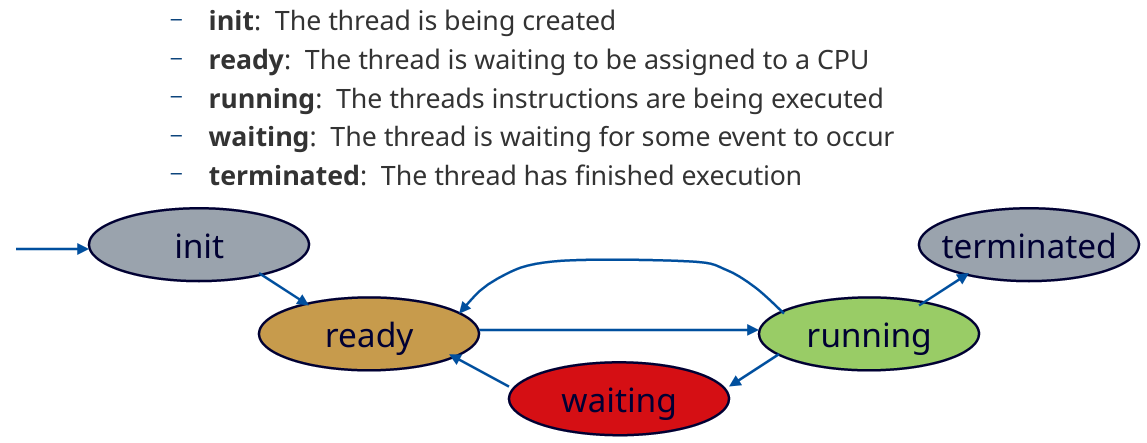
\includegraphics[width=0.7\linewidth]{Pictures/scheduling_dia}
\end{figure}

\subsection{When are scheduling decisions made?}
Am Ende von jedem Quantum. Welcher Thread als n\"achstes in \textbf{running} darf. Immer wenn ein neuer thread im system ankommt.

\subsection{What are the optimiztion criteria of a scheduler?}
\begin{itemize}
	\setlength\itemsep{-0.5em}
	\item Resposivit\"at
	\item Durchsatz
	\item Wartezeit
	\item Turn Arount Time(Zeit vom ersten Ausf\"uhren eines Threads bis zum letzten Ausf\"uhren)
	\item Auslast der CPU 
\end{itemize}

\subsection{Draw a FIFO Gantt Chart for the given taskset. Assume a context switch takes no time.}
\begin{figure}[H]
	\centering
	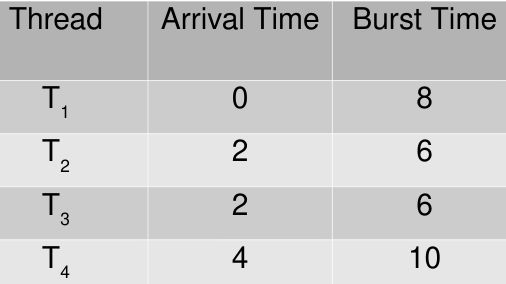
\includegraphics[width=0.25\linewidth]{Pictures/scheduling_gantt_table_fifo}
\end{figure}
\begin{figure}[H]
	\centering
	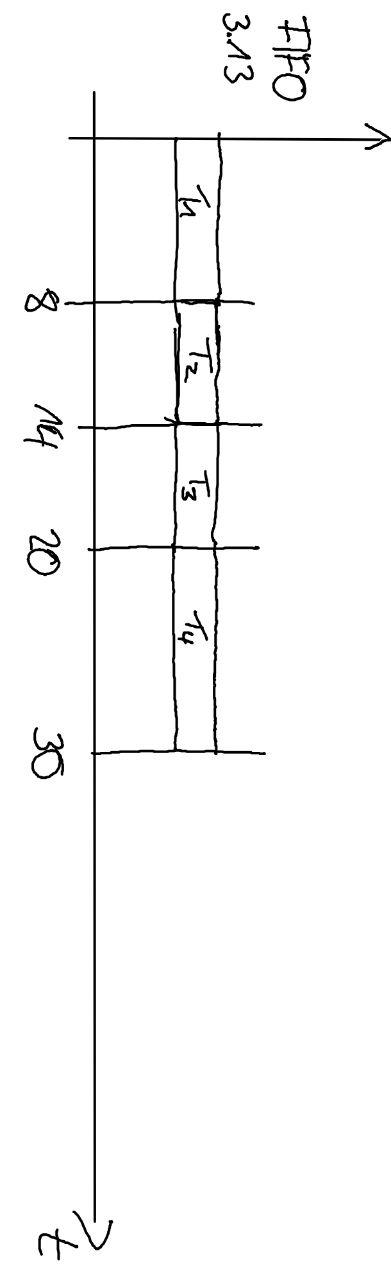
\includegraphics[width=0.25\linewidth,angle=90,origin=c]{Pictures/scheduling_gantt_dia_fifo}
\end{figure}

\subsection{Draw a Round Robin Gantt chart for the given taskset. Assume a context switch takes not time, use quantum of length 3}
\begin{figure}[H]
	\centering
	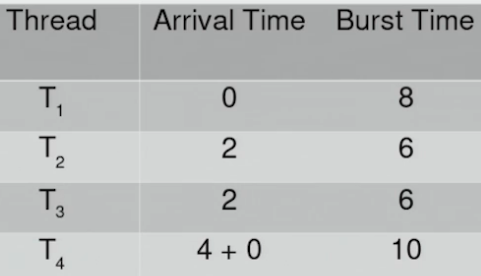
\includegraphics[width=0.25\linewidth]{Pictures/scheduling_gantt_table_rr}
\end{figure}
\begin{figure}[H]
	\centering
 	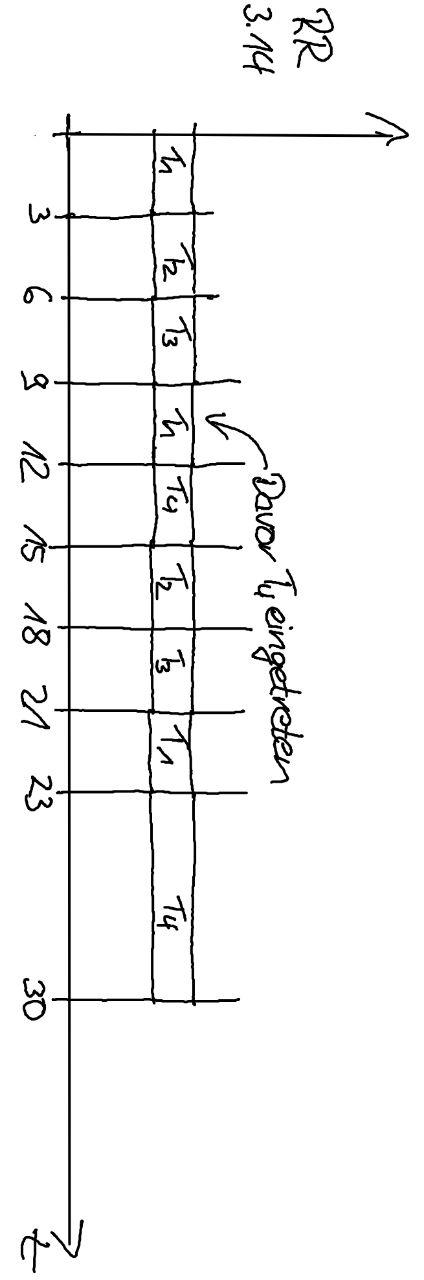
\includegraphics[width=0.25\linewidth,angle=90,origin=c]{Pictures/scheduling_gantt_dia_rr}
\end{figure}

\subsection{Draw a Round Robin Gantt chart for the given taskset. Assume a context switch takes not time, use quantum of length 3}
\begin{figure}[H]
	\centering
	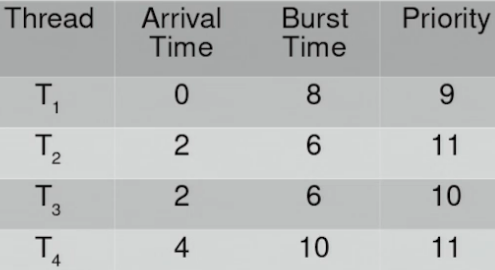
\includegraphics[width=0.25\linewidth]{Pictures/scheduling_gantt_table_rr_prio}
\end{figure}
\begin{figure}[H]
	\centering
	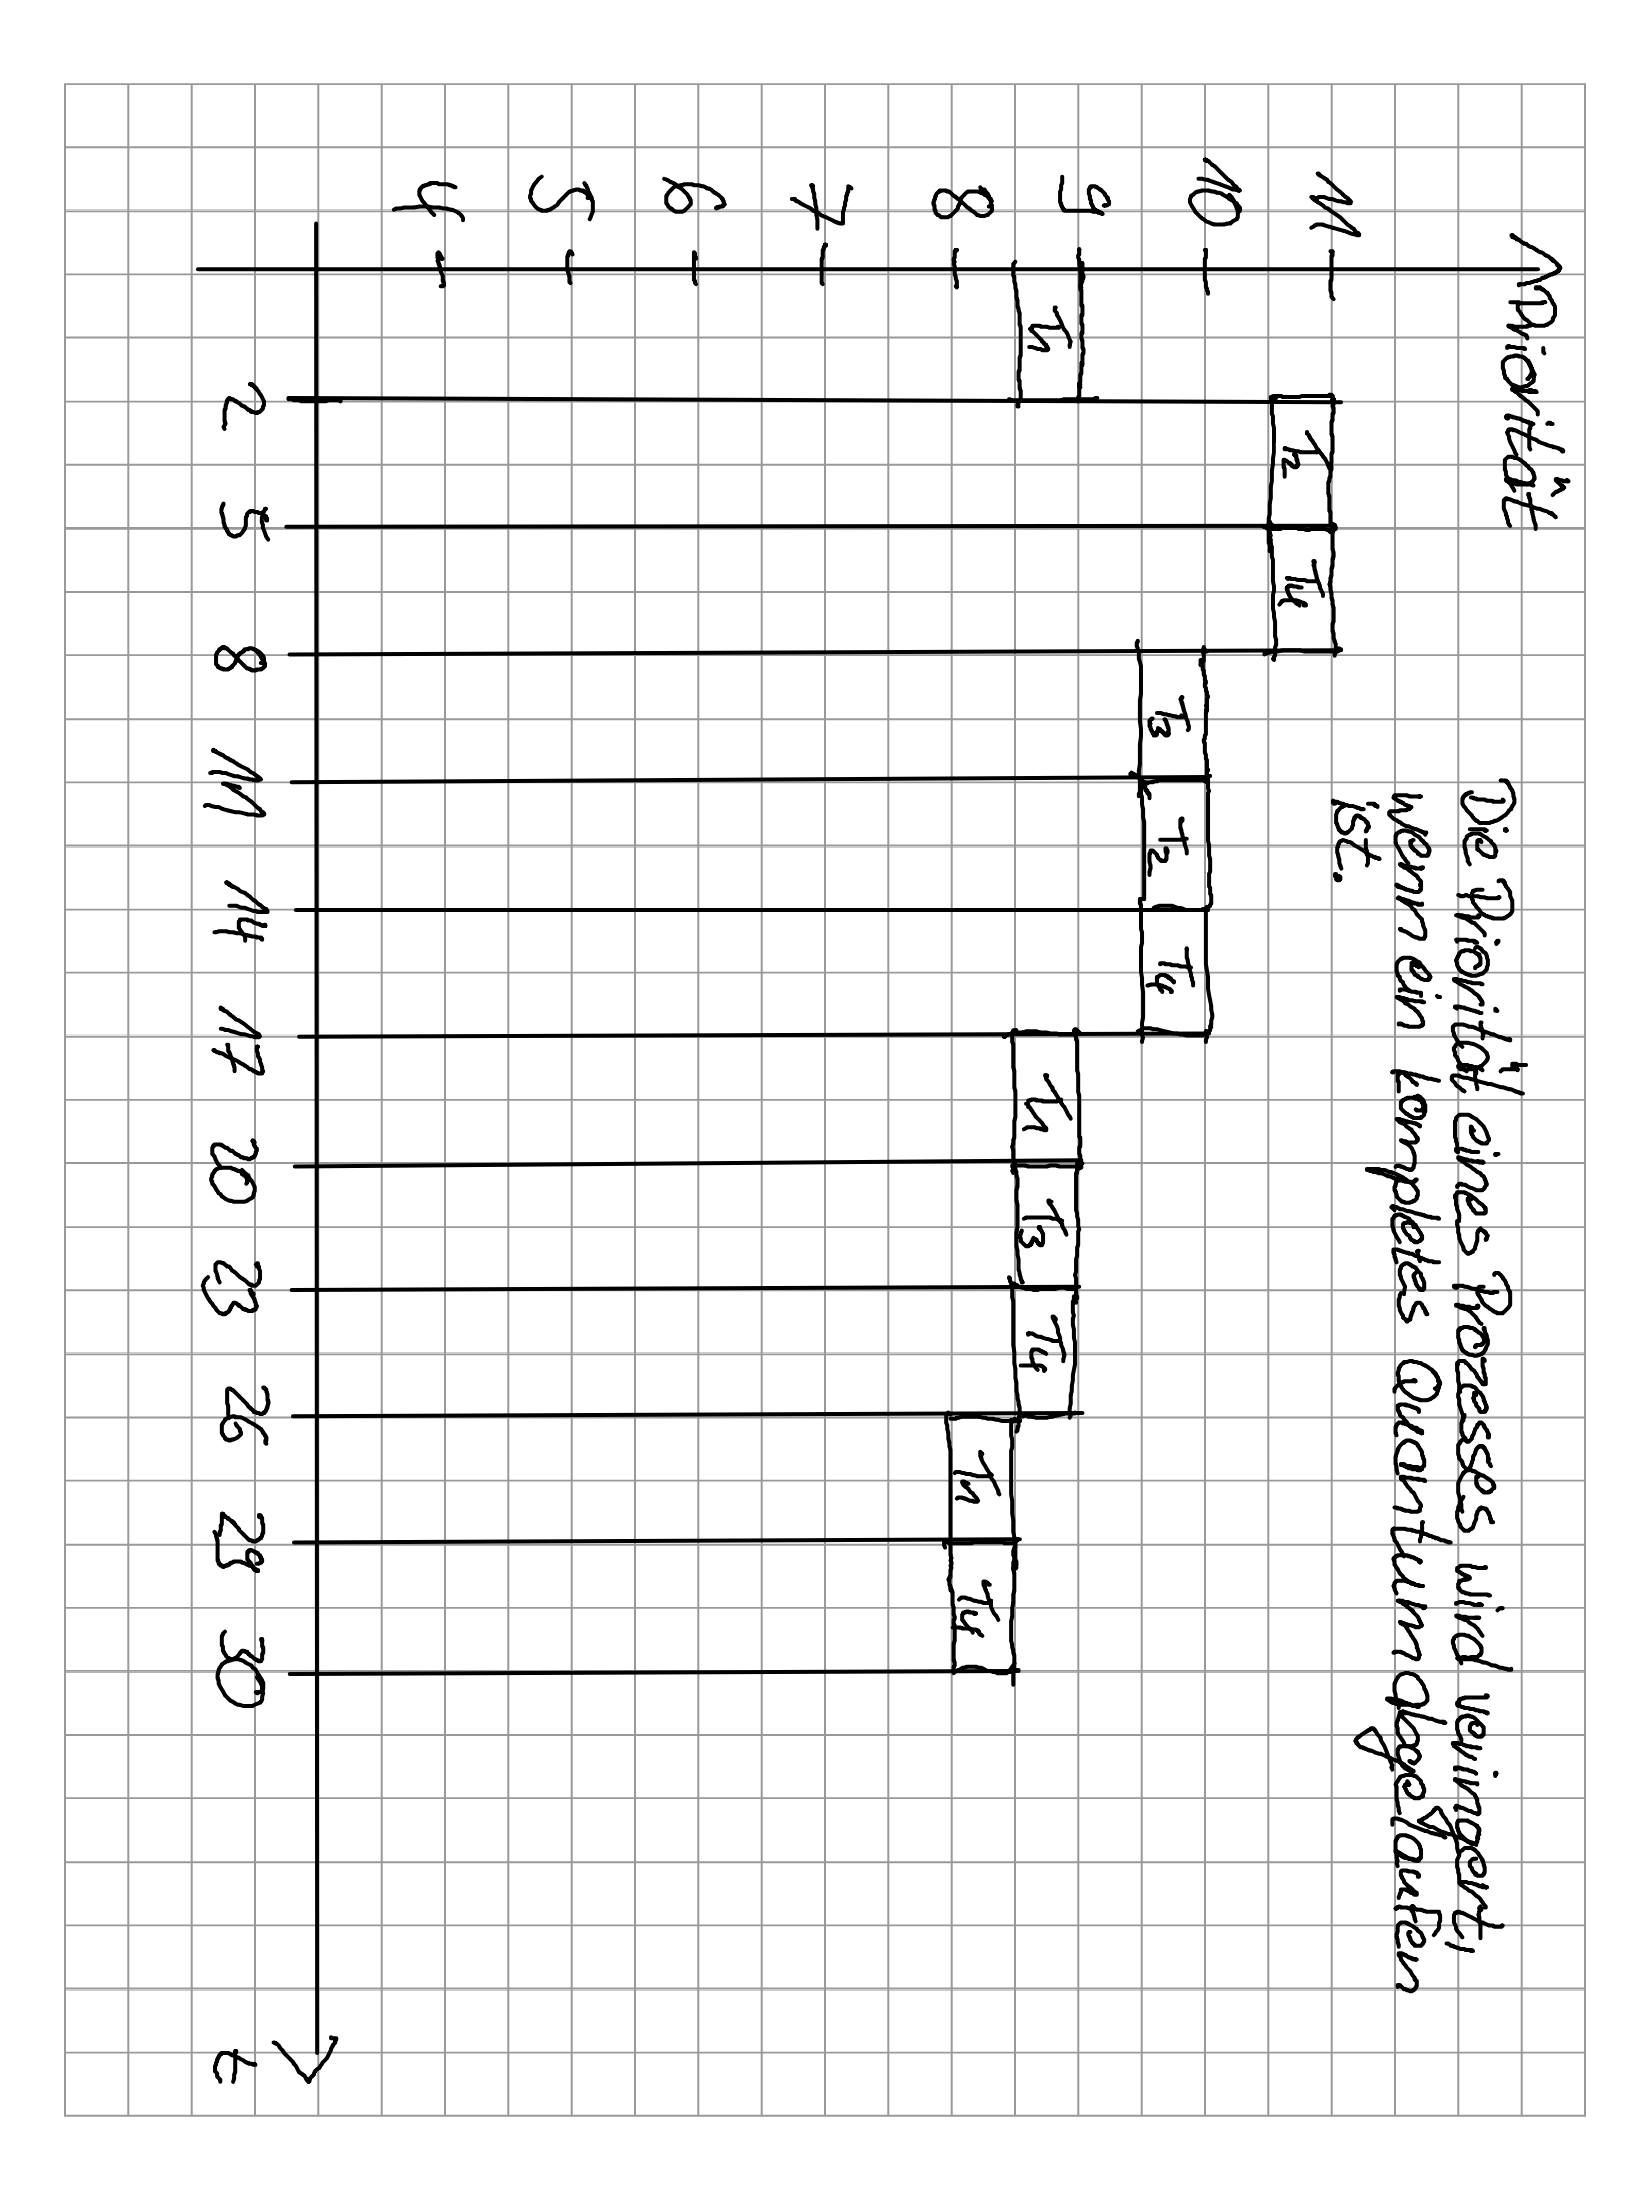
\includegraphics[width=0.6\linewidth,angle=90,origin=c]{Pictures/scheduling_gantt_dia_rr_prio}
\end{figure}

\subsection{Calculate for each thread waiting time, turnaround time, throughput and compare}
\begin{itemize}
	\setlength\itemsep{-0.5em}
	\item \textbf{waiting time} eintreten in die Queue bis zur Ausf\"uhrung der ersten Instruktion
	\item $Time Of First Instruction - ArrivalTime = WaitingTime$
	\begin{multicols}{3}
	\item FIFO
	\begin{itemize}
		\item $T_1=0$
		\item $T_2=8-2=6$
		\item $T_3 = 14-2=12$
		\item $T_4 = 20-4=16$
	\end{itemize}
	\columnbreak
	\item RR
	\begin{itemize}
		\item $T_1 = 0$
		\item $T_2 = 3-2=1$
		\item $T_3 = 6-2=4$
		\item $T_4 = 12-4=8$
	\end{itemize}
	\columnbreak
	\item RR + Prio
	\begin{itemize}
		\item $T_1 = 0$
		\item $T_2 = 0$
		\item $T_3 = 8-2=6$
		\item $T_4 = 5-4=1$
	\end{itemize}
	\end{multicols}
	\item	\textbf{Turn Around Time} Zeit die der Task im System verbringt
	\begin{multicols}{3}
		\item FIFO
		\begin{itemize}
			\item $T_1= Burst = 8$
			\item $T_2=Burst=6$
			\item $T_3 =Burst=6$
			\item $T_4 =Burst=10$
		\end{itemize}
		\columnbreak
		\item RR
		\begin{itemize}
			\item $T_1 = 23$
			\item $T_2 = 18-3=15$
			\item $T_3 = 21-6=15$
			\item $T_4 = 30-12=18$
		\end{itemize}
		\columnbreak
		\item RR + Prio
		\begin{itemize}
			\item $T_1 = 29$
			\item $T_2 = 14-2=12$
			\item $T_3 = 23-8=15$
			\item $T_4 = 30-5=25$
		\end{itemize}
	\end{multicols}
	\item \textbf{response time} Eintritt in die Warteschlange bis zur erste Antwort des BS.
	\item \textbf{throuput} Menge der Threads pro Zeiteinheit. Hier: 4 Threads/30 Zeiteinheiten(auf Grund der Annahme, Kontextwechsel==0 !)
\end{itemize}

\subsection{Describe the problem of thread starvation in relation to priority schedulers.}
Ein Thread mit hoher Priorit\"at h\"alt einen Thread mit niedriger Priorit\"at vom laufen ab.

\subsection{What is a multilevel queue scheduler? Linux and Windows both contain multilevel queue schedulers. Name an example for a queue level and describe what properties threads in this queue have.}
Scheduler der mehrere queues hat. In einander verschachtelt.\\
Windows: 16 Prios + 16 Realtime Prios (Algorithmen)\\
Linux: FIFO, RR + Batch, Idle\\
\missing\\
\unsure

\subsection{Name 2 functions related to process or thread creation.}
Linux: PThreadcreate(), fork()\\Windows: CreateProcess(), CreateThread()
\subsubsection{Name 2 functions related to process or thread termination.}
Linux: exit(), pthreadexit()\\Windows: kill(), abort()

\subsection{Compare the Linux semantics of process creation (fork/exec) to the windows semantics of process creation (CreateProcess).}
Linux fork(), exec() habe ich 2 Funktionen in den ich Sachen machen kann.\\
Windows in CreateProcess kann ich keine Sachen machen und ich habe nur eine Funktion. Parameter\"ubergabe f\"ur Pipes als Argument integriert.

\subsection{What are the advantages and disadvantages of multithreading in a programm?}
Wir m\"ussen unsere geteilten Resourcen vor einander sch\"utzen. Wir k\"onnen eine h\"ohere Auslastung des Systems erreichen.

\subsection{Compare User Mode Threads to Kernel Mode Threads. When would you use which?}
Kernel Mode Threads sind Threads die wirklich auf Threads im Kernel abbilden. Umgekehrt f\"ur User Mode Threads.

\subsection{What are Fibers?}
\begin{itemize}
	\setlength\itemsep{-0.5em}
	\item[a:] User Mode Threads on Windows
	\item[b:] The Windows equivalent of UNIX pipes
	\item[c:] Units of time counted in the Linux Kernel
	\item[d:] Users in a traditional UNIX system
\end{itemize}
Antwort \textbf{A}

\subsection{What are cgroups?}
\begin{itemize}
	\setlength\itemsep{-0.5em}
	\item[a:] groups of capabilities of an executable
	\item[b:] groups of redundant file system entries
	\item[c:] isolated process control groups in Linux
	\item[d:] groups of users in Windows
\end{itemize}
Antwort \textbf{C}: Prozessgruppen die voneinander isoliert werden. Bsp. Docker

\subsection{Describe the specific challenges of real-time scheduling. What is the difference between soft and hard real-time?}
Software die mit Deadlines umgehen k\"onnen muss. Soft: Dienst degradiert Bsp. Youtube, Hard: Autokontrolle, Flugzeugkontrolle $\rightarrow$ Unfall, Katastrophe\\
Sehr schwierig, weil man kann die Verz\"ogerungen nicht im Vorraus kennen(Caches, Interrupts)

\subsection{Describe one of the three discussed approaches of starvation avoidance.}
PrioBoosting on Windows\\PrioAgeing, Niceness on Linux\\
PrioBoosting: Thread bekommt kurz eine sehr hohe Prio sinkt dann aber wieder ab\\
PrioAgeing: Threads werden St\"uck f\"ur St\"uck abgesenkt

\subsection{What is priority inversion?}
Thread mit niedriger Prio h\"alt Thread mit hoher Prio vom laufen ab $\rightarrow$ Locks\\

\begin{figure}[H]
	\centering
	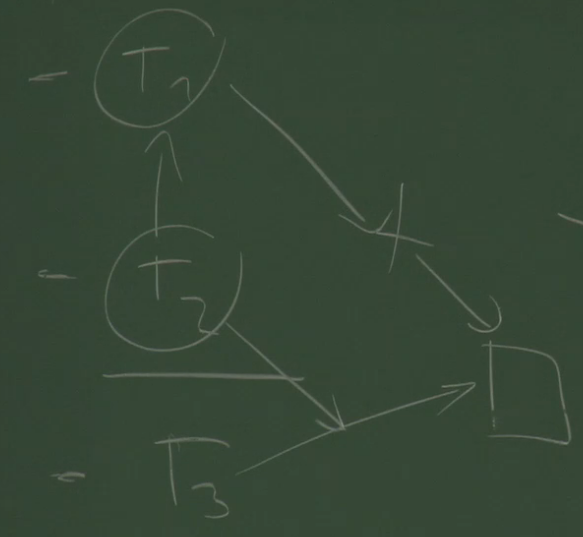
\includegraphics[width=0.5\linewidth]{Pictures/priority_inversion}
\end{figure}

\subsection{Which of the following is not a queue level in Completely Fair Scheduler (CFS)?}
\begin{itemize}
	\setlength\itemsep{-0.5em}
	\item[a:] SCHED\_BATCH
	\item[b:] SCHED\_HIGH
	\item[c:] SCHED\_RR
	\item[d:] SCHED\_FIFO
\end{itemize}
Antwort \textbf{b}: ist Ausgedacht von dem Dozenten

\subsection{Describe the concept of niceness in relation to the Linux Completely Fair Scheduler (CFS).}
Wir haben einen relativen Wert zwischen $\pm$20. Der Wert beschreibt das Verh\"altnis L\"ange der Ausf\"uhrungszeit, die die Threads zu einander bekommen mit einer Nicewert Differenz von ca 1,25 entsprechend der Laufzeit.\\Ein Thread der 1 niedrigeren Nicewert hat als ein anderer Thread, wird 1,25 mal so lange ran kommen.

\subsection{What is thread affinity? Compare hard affinity and soft affinity.}
Bitmaske, welche auf einem Multicore System festlegt auf welchen Core ich laufen darf. Ich darf auf den Kernen laufen, auf denen meine Affinit\"atsmaske eine 1 hat.\\
Bei harter Affinit\"at kann dies manuell eingestellt werden.\\
Bei softer Affinit\"at wird dem Thread zu erst der Core zugewiesen, welcher am besten ist. Beim Fortsetzen wird versucht wieder diesen Core zu benutzen da hier alle Daten schon vorhanden sind.

\subsection{On a high level, outline the similarities and differences of the Windows and Linux Scheduler.}
Gemeinsamkeiten: Priorit\"aten\\
Linux: Nicewerte\\
Windows: \\
$\dots$\\
\missing
\section{Checkpoint 4}

% align with slide numbers
\addtocounter{subsection}{1}

\subsection{What is the role of the Memory Management Unit (MMU)}
Sie übersetzt logische (Adresse im Programm) auf physikalische Adressen (Adresse auf Festplatte).
(Passiert bei jedem Speicherzugriff neu.)

\subsection{What is the difference between virtual / logical Adresses and physikal adresses?}

\subsection{What is Segmentation?}

\subsection{What are the main shortcommings of Segmentation?}

\subsection{Describe Paging. How is it different from Segmentation, and how does it address the shortcumings of Segmentation?}

\subsection{Describe the layout of a Page Table. Why do some architectures use multi-level page table structures?}

\subsection{Name two bits associated with each Page Table Entry and describe their purpose.}

\subsection{What is the role of the Translation Lookaside Buffer (TLB)?}

\subsection{Assume a memory system that manages adresses of 26 bits length, with a page size of 256 bytes. How many entries does a page table have?}

\subsection{What is the size of the virtual adress space?}

\subsection{How long are the adresses page number and offset?}

\subsection{Each page table entry has two status bits.}

\subsection{What is the length of a page table entry?}

\subsubsection{What is the total size of a page table?}

\subsection{Assume the described system has access to 24MiB of physical memory, half of which is reserved for the operating system. Of this half, 5MiB are reserved for process page tables, and are not pageable. How many processes can this system support?}

\subsection{What is the maximum size of a process working set, assuming that no reserved OS pages are part of the working set?}

\subsection{What is a Page Fault?}

\subsection{What is the difference between a Soft Page Fault and a Hard Page Fault?}

\subsection{Name two different reasons for which a memory access coul produce a Page Fault.}

\subsection{What is a Working Set?}

\subsection{What is the role of the Modified, Standby, Free, Zero and Bad Page Lists? What properties do pages in these lists have? How do pages transition between these lists?}

\subsection{What is the purpose of the Page Frame Number Database?}

\subsection{Describe the page replacement algorithms First-In-First-Out (FIFO), Second Chance, and Least-Recently-Used (LRU).}

\subsection{What is Béládys Anomaly, as found in the FIFO page replacement algoritm?}

\subsection{Assuming three frames of physical memory, and a memory access pattern to the virtual pages: 2,1,4,2,3,4,2,1,3,4,3. How many Page Fault would FIFO incur?}

\subsection{How many Page Faults would Second Chance incur?}

\subsection{How many Page Faults would LRU incur?}

\subsection{What is the difference between swapping and page replacement (paging)?}

\subsection{Describe the difference between reserved and committed memory.}

\subsection{What is a Guard Page? What could it be used for?}

\subsection{How do operating systems implement shared memory?}

\subsection{What is Copy-on-Write (CoW) memory, and what is it used for?}


\renewcommand{\indexname}{Stichwortverzeichnis} 

% Stichwortverzeichnis soll im Inhaltsverzeichnis auftauchen 
\addcontentsline{toc}{section}{Stichwortverzeichnis} 

% Stichwortverzeichnis endgueltig anzeigen 
\idxlayout{columns=3}
\printindex

\end{document}